\documentclass[12pt]{article}

\usepackage[utf8]{inputenc}
\usepackage{amsmath,amssymb,amsthm}
\usepackage{graphicx}               
\usepackage{hyperref} 
\usepackage{amsmath}


\title{Assignment 1 \\\vspace{1in}}


\author{Andrew Ungureanu \\
        40283344\\\vspace{1in}}
\date{Tuesday, March 4th 2025\\
            SOEN 331}

\begin{document}

\maketitle

\newpage
\section*{Problem 1: Propositional Logic (7 pts)}

\subsection*{1.1 (3 pts)}
\textit{$P$: Humans are nice to Sofia\\
$Q$: Sofia is nice to humans}
\text{$P \rightarrow Q$}
\begin{itemize}

    \item  $P \rightarrow Q$ If humans are nice to Sofia, then Sofia is nice to humans.
    \item $\neg P$ Humans are not nice to Sofia.
    \item Therefore, $\neg Q$ Sofia is not nice to humans.
\end{itemize}
\begin{center}
    \begin{tabular}{|c|c|c|}
        \hline
        $P$ & $Q$ & $P \rightarrow Q$ \\
        \hline
        T & T & T \\
        T & F & F \\
        F & T & T \\
        F & F & T \\
        \hline
    \end{tabular}
\end{center}

As seen from this truth table, it is not implied that when humans are not nice, then Sofia will not be nice to humans. Indeed, there are two possibilities for it. Therefore, there is an inverse error and you can not determine Sofia is a threat to humans.


\subsection*{1.2\,(4 pts)}
\textit{}{$P$: Each man has a definite set of rules of conduct
\\$Q$: Man is no better than a machine}
\begin{itemize}

    \item  $P \rightarrow Q$ If men have strict rules, then they are like machines.
    \item $\neg P$ There are no such rules.
    \item Therefore, $\neg Q$ Men cannot be machines.
\end{itemize}

This argument follows once again falls in the inverse error category, which is an invalid form of reasoning. In general, from $P \rightarrow Q$ and $\neg P$, we cannot logically conclude $\neg Q$.


\newpage
\section*{Problem 2: Predicate logic (8 pts)}

\subsection*{2.1 \,(4 pts)}
\begin{enumerate}
    \item[(a)] $\forall x \in \mathbb{R} : \text{number}(x) \rightarrow \neg \text{rational}(x)$ \\
    \textit{For all $x$, if $x$ is a real number, then $x$ is not rational.} \\
    \textbf{Type: E}
    \item[(b)] $\exists x \in \mathbb{R} : \text{number}(x) \land \text{rational}(x)$ \\
    \textit{There exists a number that is real and rational.} \\
    \textbf{Type: I}
\end{enumerate}

\subsection*{2.1 \,(4 pts)}

\begin{enumerate}
    \item[(a)] $\forall x \in \mathbb{R}, \text{number}(x) \rightarrow \text{rational}(x)$ \\
    \textbf{Type: E}
    \item[(b)] $\exists x \in \mathbb{R}, \text{number}(x) \wedge \neg \text{rational}(x)$ \\
    \textbf{Type: I}
\end{enumerate}
\newpage

\section*{Problem 3: Linear Temporal Logic 1 (15 pts)}

\subsection*{3.1 (3 pts)}

\begin{equation*}
    \bigcirc \Box (\phi \oplus \psi) \rightarrow \bigcirc^2 \Diamond (\chi W \tau)
\end{equation*}

\subsection*{3.2 (3 pts)}


\begin{equation*}
    (\phi \oplus \psi) \rightarrow \bigcirc \Box (\chi \rightarrow (\kappa R \omega))
\end{equation*}

\subsection*{3.3 (3 pts)}
\begin{equation*}
    \neg (\neg \varphi \vee \neg \psi) \rightarrow \Diamond \Box \tau \land \bigcirc^2 \Diamond \pi
\end{equation*}

\begin{figure}[h]
    \centering
    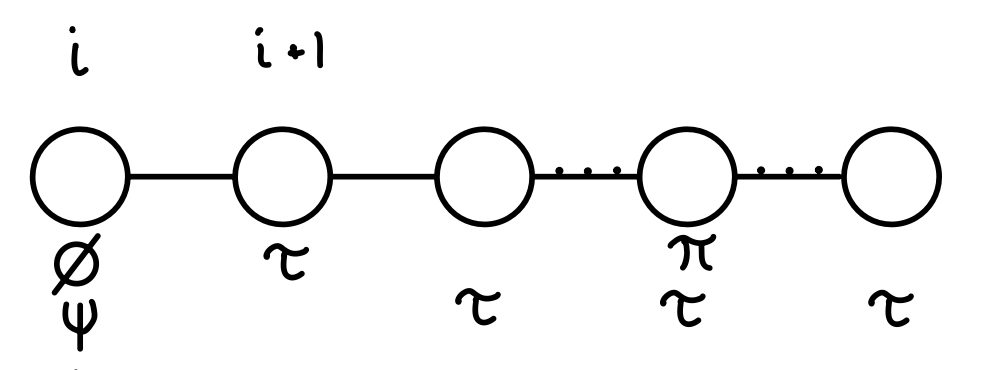
\includegraphics[width=0.7\textwidth]{images/3.3}
\end{figure}

If $\varphi$ and $\psi$ are true, then $\tau$ will eventually become invariant and starting from time $i+2$, $\pi$ will eventually happen.

\subsection*{3.4 (3 pts)}
\begin{figure}[h]
    \centering
    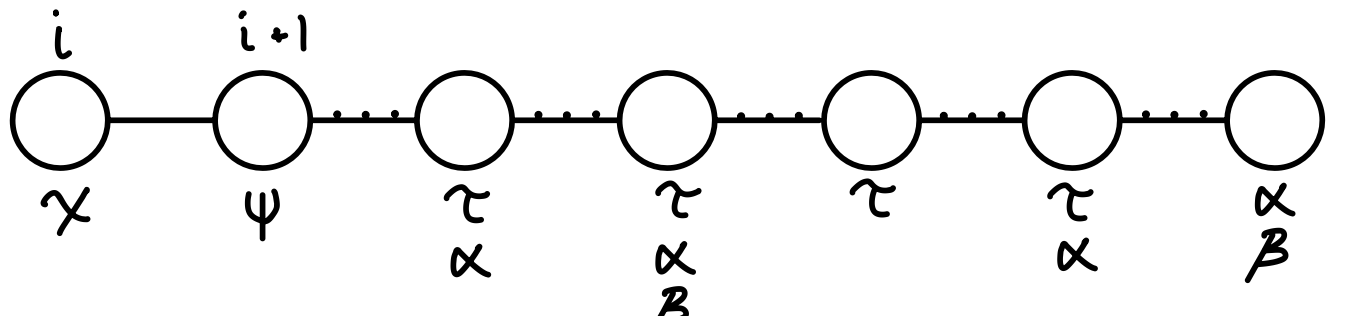
\includegraphics[width=0.9\textwidth]{images/3.4}
\end{figure}
If starting at time $i+2$, $\tau$ eventually becomes invariant and at time $i$, x becomes true and $/psi$ becomes true at time $i+1$, then starting at time $i+2$, $\tau$ will be true at all states until and including when $\beta$ becomes true, infinitely often. 


\subsection*{3.5 (3 pts)}
\begin{figure}[h]
    \centering
    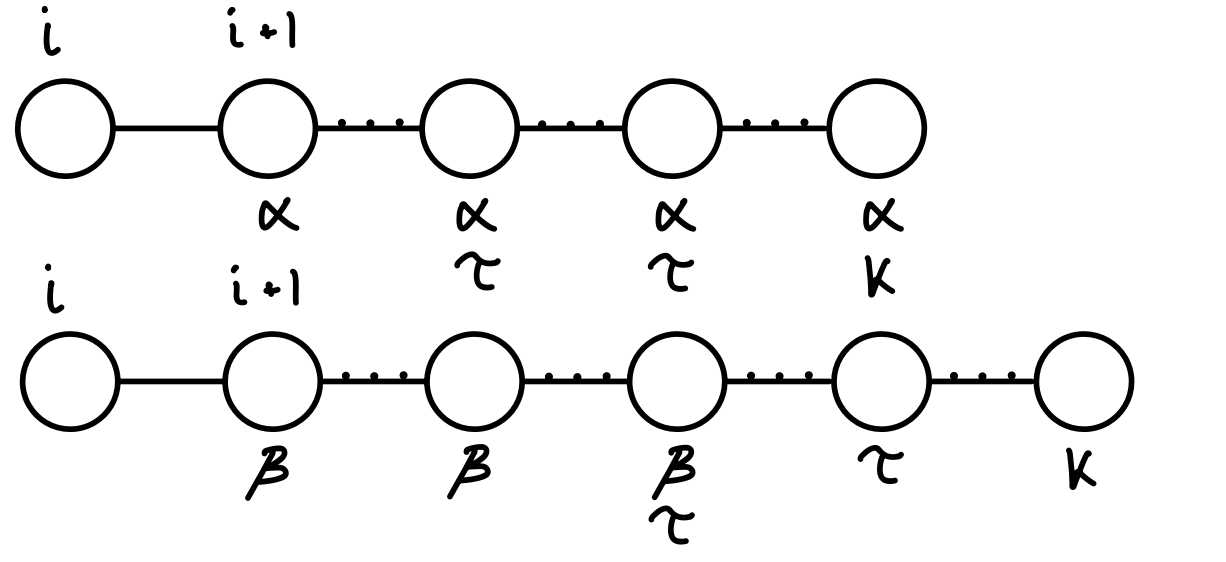
\includegraphics[width=0.7\textwidth]{images/3.5.png}
\end{figure}
If at time $i+1$, either one but not both of $\alpha$ and $\beta$ are true, then starting at time $i+1$, $\tau$ will eventually be true and remain until $\kappa$ becomes true. ($\kappa$ will become true)

\newpage
\section*{Problem 4: Linear Temporal Logic 2 (15 pts)}

\subsection*{4.1 Visualizing all models of behavior \,(9 pts)}
\begin{figure}[h]
    \centering
    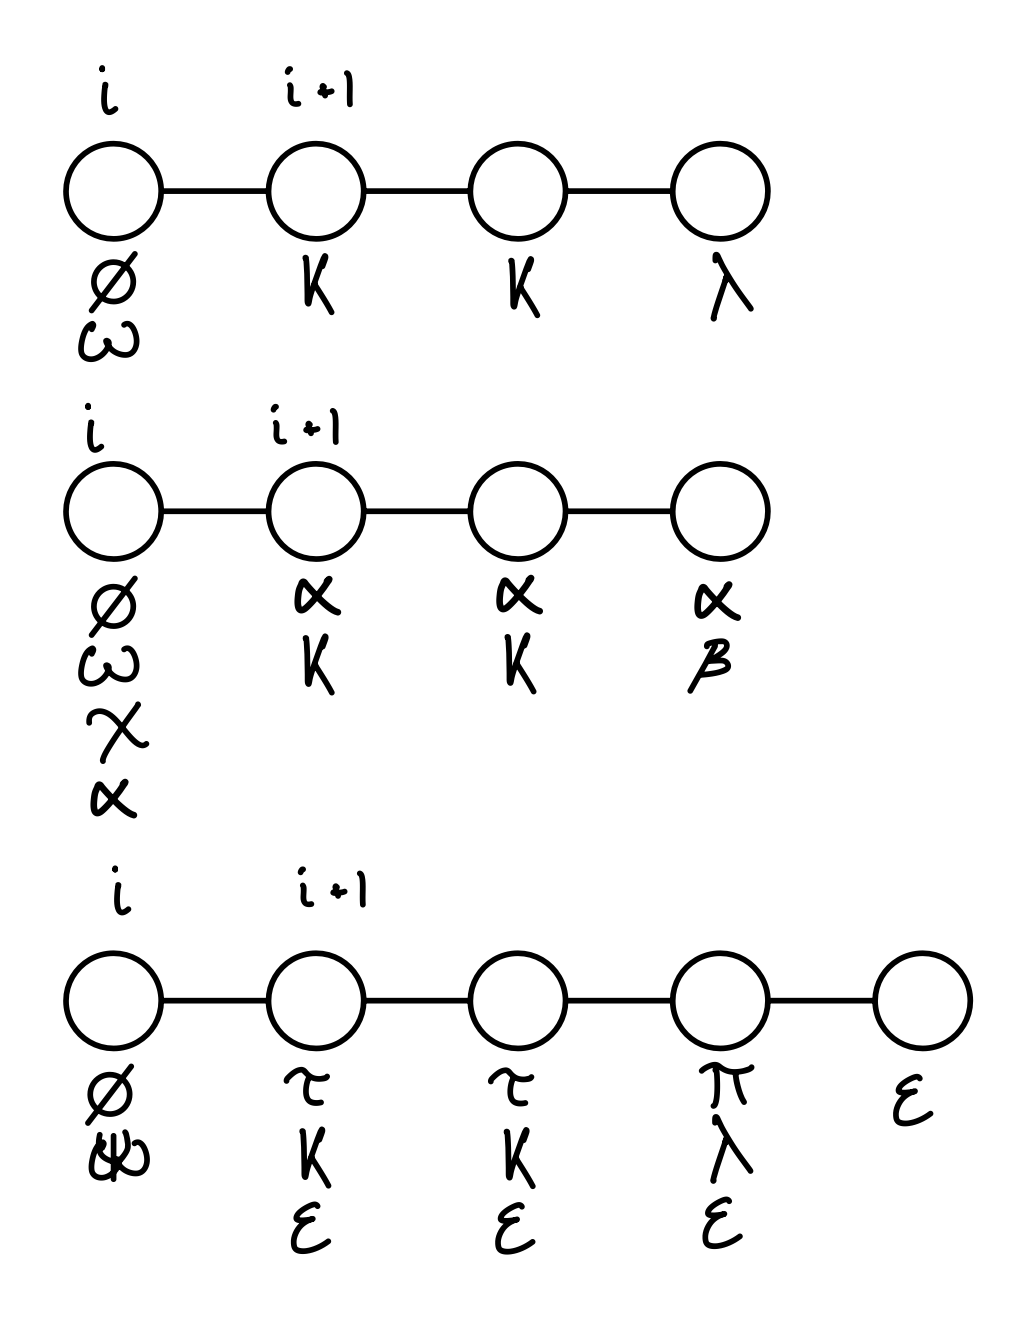
\includegraphics[width=0.5\textwidth]{images/4.1}
\end{figure}

\subsection*{4.2 \,(4 pts)}
\begin{align*}
    &\langle (\phi \wedge \omega), \kappa, \kappa, \lambda \rangle \\
    &\langle (\phi \wedge \chi \wedge \omega \wedge \alpha), (\alpha \wedge \kappa), (\alpha \wedge \kappa), (\alpha \wedge \beta \wedge \lambda) \rangle \\
    &\langle (\phi \wedge \psi \wedge \omega), (\tau \wedge \kappa \wedge \epsilon), (\tau \wedge \kappa \wedge \epsilon), (\pi \wedge \lambda \wedge \epsilon), \epsilon \rangle
\end{align*}

\subsection*{4.3 \,(2 pts)}
Model 1: The first model fully terminates. Additionally, it is consistent.
Model 2: The second model fully terminates. Additionally, it is consistent.
Model 3: The third model fully terminates. Additionally, it is consistent.
\newpage
\section*{Problem 5: Unordered Structures (10 pts)}
\begin{enumerate}
    \item \textit{Crew = $\mathbb{P}$ Names}
    \item \textit{Spock} would not be a legitimate value, as all values of \textit{Crew} must be a set of names. \textit{Spock} is not (it does not have curly braces).
    \item \textit\{Kirk\} is a valid subset of \textit{Names}. In $\mathbb{P}$ Names, it is the set of all subsets of S. \{Kirk\} is one of those subsets which makes this valid.
    \item No, it is not. Writing \textit{Crew: $\mathbb{P}$ Names} is interpreted as the variable \textit{Crew} can assume any value supported by the Powerset of \textit{Names}. However, \textit{Crew = $\mathbb{P}$ Names} means that the variable Crew is the Powerset of \textit{Names}.
    \item No, the elements in \textit{Names} aren't sets. Therefore, they can't be subsets of \textit{$\mathbb{P}$ Names} if they are individual names.
    \item \textit{\{Names\} = \{\{Kirk, Spock, ...\}\}} is not an element of Powerset of \textit{Names}.
    \item No, the elements of the product are actually ordered pairs.
    \item Yes, because ever Powerset has an empty set.
    \item The variable \textit{Commander} can assume any value supported by the Powerset of \textit{Crew}. For example, can be the empty set \{\}, one element of the said or the entire set.
    \item They must be ordered pairs. Therefore, in this case it is false.
\end{enumerate}
\newpage
\section*{Problem 6: Ordered Structures (10 pts)}

\subsection*{6.1\,(4 pts)}

To implement a Queue Abstract Data Type with element  $\langle 1,2,3 \rangle$, I would utilize the Stack data type. However, these two different data types operate differently. Queues work with the priniciple of first-in and first-out. Stacks work by adding removing elements from the same end. Therefore, using two lists of stacks will help us modify this difference by utilizing the push and pop operations. In addition, this proposed model will allow us to have elements of generic type T.

\subsection*{6.2\,(6 pts)}
You define two lists L1 and L2 which are both stacks and have the proprieties of a stack\\
\textbf{Enqueue: Add an element to the back of a line}
\begin{itemize}
    \item To add an element to the queue, simply push it onto L1:
    \begin{equation*}
        L1.push(el)
    \end{equation*}
\end{itemize}
\textbf{Dequeue: Remove first element of a line}
\begin{itemize}
    \item To remove an element, we need to reverse the order:
    \begin{enumerate}
        \item Move all elements from L1 to L2 using:
        \begin{equation*}
            L2.push(L1.pop()) \quad \text{(repeat until L1 is empty)}
        \end{equation*}
        \item Remove the top element from L2:
        \begin{equation*}
            L2.pop()
        \end{equation*}
        \item Move all elements back from L2 to L1:
        \begin{equation*}
            L1.push(L2.pop()) \quad \text{(repeat until L2 is empty)}
        \end{equation*}
    \end{enumerate}
\end{itemize}

This ensures that elements are dequeued in the correct order while still using stack operations.


\newpage
\section*{Problem 7: Binary Relations, Functions, and Orderings (15 pts)}

\subsection*{7.1}
*LACK OF TIME


\subsection*{7.2\,(1 pts)}
*LACK OF TIME

\subsection*{7.3\,(12 pts)}
\begin{itemize}
    \item a) The variable \(map\) is a function. It is a partial function because not the element 2 does not have a corresping element in the codomain. The domain is \(\{2, 4, 6, 24, 36, 72\}\), and the codomain is the power set of \(\{1, 2, 3\}\).
    \item b) \begin{itemize}
       \item \textbf{Injective:} No, because multiple domain elements map to the same set (36 and 6 \(\{3\}\)).
       \item \textbf{Surjective (Onto):} No, because not every subset of \(\{1, 2, 3\}\) is mapped.
       \item \textbf{Bijective:} No, because it is not injective or surjective.
       \item \textbf{Order Preserving:} No, because the order of elements in the domain is not preserved in the codomain.
       \item \textbf{Order Reflecting:} No because order is not preserved as previously stated.
       \item \textbf{Order Embedding:} No, as it does not preserve or reflect order.
       \item \textbf{Isomorphism:} No, because it is not bijective and does not preserve structure.
\end{itemize}
\end{itemize}


\newpage
\section*{Problem 8 Binary Relations, Functions and Orderings 2 (10
pts)}
(a) The variable \(map2\) is a function. It is a total function because every element in the domain has a corresponding element in the codomain. The domain is \(\{\{1,2,3\}, \{1,2\}, \{1,3\}, \{2,3\}, \{1\}, \{2\}, \{3\}\}\), and the codomain is \(\{2, 3, 4, 6, 24, 36, 72\}\).

(b) 
\begin{itemize}
       \item \textbf{Injective (One-to-One):} No, because different subsets map to the same value.
       \item \textbf{Surjective (Onto):} Yes, because every element in the codomain is mapped to by some subset in the domain.
       \item \textbf{Bijective:} No, because it is not injective
       \item \textbf{Order Preserving:} No, because the order of subsets in the domain is not preserved in the codomain.
       \item \textbf{Order Reflecting:} No, for similar reasons as order preserving.
       \item \textbf{Order Embedding:} No, as it does not preserve or reflect order.
       \item \textbf{Isomorphism:} No, because it is not bijective.
\end{itemize}


\newpage
\section*{Problem 9: Construction Techniques (10 pts)}

\subsection*{9.1\,(5 pts)}
\begin{itemize}
    \item a) 
    \begin{equation*}
    \text{cons}(f(a), \text{map}(f, \langle b, c \rangle))
    \end{equation*}
    \item b)
    \begin{equation*}
    \text{map}(f, \Lambda) = \langle \rangle
    \end{equation*}
    \begin{equation*}
    \text{map}(f, \Lambda) = \text{cons}(f(\Lambda), \text{map}(f, \text(\Lambda))
    \end{equation*}
    \item c)
    \begin{align*}
    &= \text{cons}(f(a), \text{map}(f, \langle b, c \rangle)) \\
    &= \text{cons}(f(a), \text{cons}(f(b), \text{cons}(f(c), \langle \rangle))) \\
    &= \langle f(a), f(b), f(c) \rangle
\end{align*}
    
\end{itemize}

\subsection*{9.2\,(5 pts)}
\begin{itemize}
    \item a)
    \begin{equation*}
    \text{cons}(a, \text{insert}(c, \langle b, c, d \rangle))
    \end{equation*}
    \item b)
    \begin{equation*}
    \text{insert}(c, \Lambda) = \langle c \rangle, \quad \text{if } \Lambda \text{ is empty}
    \text{  *LACK OF TIME/NOT SURE}
    \end{equation*}

    \item c) LACK OT TIME/NOT SURE
\end{itemize}

\newpage


\end{document}
